\section{Analysis of programming paradigms}

%By analyzing the degree of support of the nine MPLs
%for programming paradigms and the application scenarios of
%different MPLs, we try to find out the connection between
%the degree of support of programming paradigms and the
%application scenarios.

Extensive research has shown that programming is about solving problems,
and that problems can be solved from a variety of perspectives
and ideas, of which the universal and proven patterns are
summarized as paradigms.
Functional Programming (FP) and Object Oriented Programming (OOP)
are the two most common, and at the same time the most important paradigms
in modern programming languages.
Therefore, these two paradigms are chosen for analysis when discussing
programming paradigms below.

\subsection{Languages, paradigms, and concepts}



\begin{table*}[hb]
    \caption{Several concepts of FP and OOP}
    \label{tab:concept}
    \begin{center}
        \begin{tabular}{cll}
            \toprule
            Paradigm & Concept & Meaning \\
            \midrule
            FP & Higher-order function & Take functions as variables, which can
            pass as parameters or return values. \\
            FP & Lambda expression & A short block of code which takes in parameters
            and returns a value. \\
            FP & Partial application & Given a function with certain parameters,
            producing another function (with fewer parameters). \\
            FP & Closure & A record stores a function together with an
            environment\cite{sussman1998scheme}. \\
            FP & Type inference & The automatic detection of the type of an
            expression at compile time. \\
            FP & Pattern matching & Dispatch branch by matching the pattern of a
            given sequence of tokens. \\
            FP & Statement as expression & Take all statements as expressions, which
            creates a definite value. \\
            OOP & Encapsulation & Hide the properties and implementation details of
            the object, and only expose the interface to the outside. \\
            OOP & Inheritance & Create classes that are built upon existing
            classes\cite{johnson1988designing}. A way of
            code reuse. \\
            OOP & Composition & Combine entities into more complex ones. A way of
            code reuse. \\
            OOP & Delegation & One entity passing something to another
            entity\cite{wilkinson2009grid}. A way of code
            reuse. \\
            OOP & Trait & A set of method conventions. Broadly including trait,
            interface, protocol and mixin. \\
            OOP & Polymorphism & Use of a single symbol to represent multiple
            different
            types\cite{cardelli1985understanding}. \\
            OOP & Everything is object & All the basic elements of a programming
            language are represented in the form of objects. \\
            \bottomrule
        \end{tabular}
    \end{center}
\end{table*}

\begin{table*}[ht]
    \caption{Degree of support for FP concept}
    \label{tab:fp}
    \begin{center}
        \begin{tabular}{cccccccc}
            \toprule
            Language & Higher-order functions & Lambda expression & Partial
            application & Closures & Type inference & Pattern matching & Statements
            as expressions\\
            \midrule
            Python     & \Checkmark & \Checkmark & Python2.5   & \Checkmark & \Checkmark & Python3.10  & ×          \\
            Java       & Java8      & Java8      & Java8       & Java8      & Java10     & ×           & ×          \\
            C++        & C++11      & C++11      & C++11       & C++11      & C++11      & C++17       & ×          \\
            JavaScript & \Checkmark & \Checkmark & ECMAScript5 & \Checkmark & \Checkmark & ECMAScript6 & ×          \\
            Go         & \Checkmark & \Checkmark & \Checkmark  & \Checkmark & \Checkmark & ×           & ×          \\
            Swift      & \Checkmark & \Checkmark & \Checkmark  & \Checkmark & \Checkmark & \Checkmark  & ×          \\
            Dart       & \Checkmark & \Checkmark & \Checkmark  & \Checkmark & \Checkmark & ×           & ×          \\
            Rust       & \Checkmark & \Checkmark & \Checkmark  & \Checkmark & \Checkmark & \Checkmark  & \Checkmark \\
            Kotlin     & \Checkmark & \Checkmark & \Checkmark  & \Checkmark & \Checkmark & \Checkmark  & \Checkmark \\
            \bottomrule
        \end{tabular}
    \end{center}
\end{table*}

Each language also realizes one or more paradigms,
and each paradigm contains a core set of concepts,
as we can see in Table~\ref{fig:concept}.
FP and OOP are programming paradigms that are commonly
available in MPLs, so the rest of our discussion is based on FP and OOP\@.
Table~\ref{tab:concept} shows several concepts in FP and OOP supported by MPLs, and the meaning of a certain concept.

\begin{figure}[htbp]
    \centerline{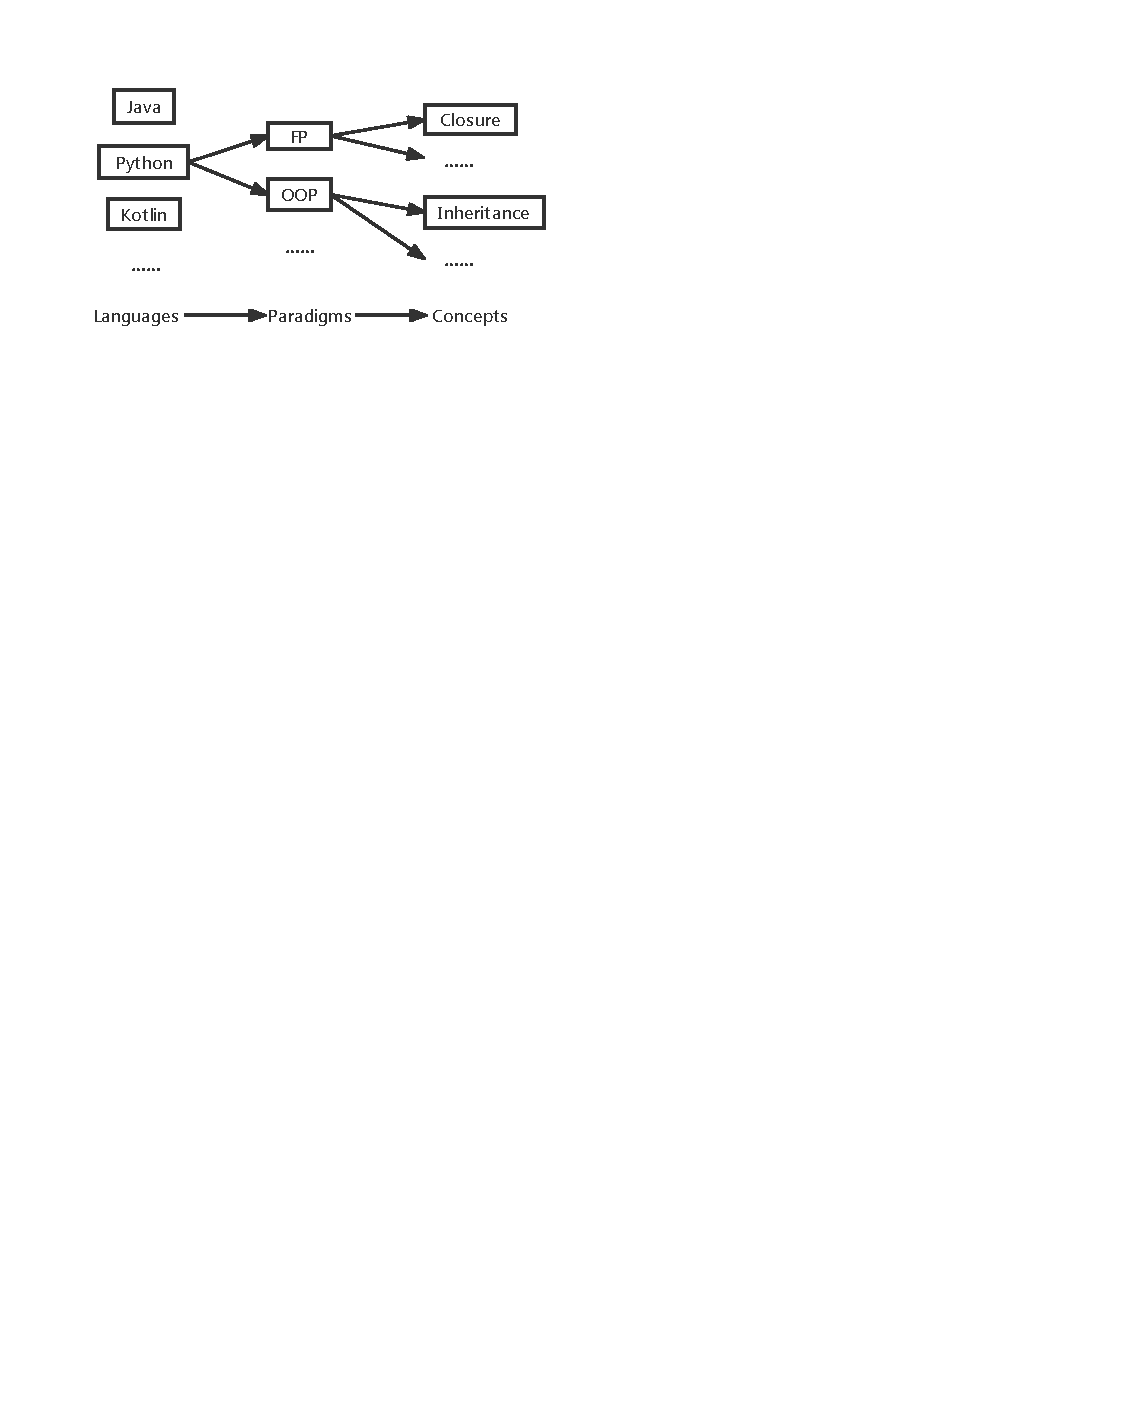
\includegraphics[scale=0.8]{figures/concept}}
    \caption{Languages, paradigms, and concepts}
    \label{fig:concept}
\end{figure}


We have adopted a more application-oriented approach to organize these concepts.
Because we tend to choose concepts defined in a particular programming
language rather than concepts from programming paradigm theory.
For example, "nested functions" and "anonymous functions" are two concepts in FP,
but in programming language implementation, "lambda expressions" supersede these two concepts.
As another example, most currently popular programming languages support "combination",
which is always an OOP concept.
When designing programming languages, the combination is simply a way of
arranging data and does not belong to any paradigm.
Even languages like the much older C provide structure combinations and
function combinations.
Therefore, the combination is not included in our analysis.

\subsection{Functional programming}

The most important feature of FP is its high degree of abstraction.
This is mainly because FP has its origins in the lambda calculus,
so it has some characteristics of abstract algebra.


As programming language practice continues to deepen,
programming languages are becoming more and more supportive
of functional concepts.
Table~\ref{tab:fp} gives the support level of the selected 9 MPLs for the concepts
of FP mentioned in Table~\ref{tab:concept}.
The right signs indicate that the programming language has
supported the concept since the language appears.
On the contrary, the wrong signs indicate that the programming language has
not supported the concept even now.
And if the programming language has supported the concept during its development,
the version that first supported the concept is indicated.


For programming languages released in the 1980s and 1990s,
their support for functional concepts was not good when they first appeared.
This is especially true for Java and C++.
From their original syntax, we can see that there is no functional concept in them.
This is because these programming languages were not designed with FP in mind.
Then, JavaScript and Python are a bit better in FP concept support.
Although they inherently support some basic functional concepts, they are missing some advanced ones.
As for the programming languages released around 2010, they all support the core functional concept.
In particular, Rust and Kotlin additionally support the concept of "statements as expressions",
a milestone in the development of MPL paradigm convergence.
The concept of "statements as expressions" provides semantic unification of expressions and statements,
and is more common in FP languages(compared to OOP).
As programming languages continue to evolve, some programming language with paradigm convergence,
like Kotlin and Rust, has supported this concept.
Thus Kotlin and Rust can be considered as having a higher level of support for FP concepts.

\subsection{Object oriented programming}
The most important feature of OOP is its emphasis on reuse. Back in the 1960s, software maintenance became increasingly difficult due to the increasing complexity of hardware and software. OOP solves this problem by emphasizing reusability. In the practice of OOP, one maps real problems into entities and their relationships, rather than being concerned with the process of dealing with the problem.

%The most important feature of OOP is its emphasis on reuse. Back in the 1960s, software maintenance became increasingly difficult due to the increasing complexity of hardware and software. OOP solves this problem by emphasizing reusability. In the practice of OOP, one maps real problems into entities and their relationships, rather than being concerned with the process of dealing with the problem. After the birth of object-oriented languages, there was an urgent need to map from problems to entities and relationships in a modeling way, at which point UML was born. It is a set of standardized modeling languages for visualization and has greatly contributed to the development of object-oriented methodologies. Since then the practice of OOP has always emphasized design before implementation.

For the core concepts of OOP, there is not much difference in the level of support of MPLs, see Table~\ref{tab:oop}.
Table~\ref{tab:oop} shows the degree of support of the selected 9 MPLs for the conception of the OOP
mentioned in Table~\ref{tab:concept}.
The meaning of the right/wrong signs in the table is the same as in Table~\ref{tab:fp}.

There are three ways to realize reuse: inheritance, combination, and delegation.
In addition, more and more programming languages are realizing object-oriented
features by supporting combinations and delegates, while mere
inheritance has proven to be bad practice\cite{gamma1995design}.
Therefore, the concept of classes and inheritance is abandoned in Go and Rust, and object orientation is realized through trait. Compared to class-based object-oriented, trait-based object-oriented has a looser coupling and more flexible realization. However, most MPLs support both trait and class for different granularity of control.

In order to more accurately distinguish the degree of OOP concept support for each MPL, some concepts that are not commonly used are introduced here. An example is "everything is object". According to the definition of OOP, it should have been the most basic concept in OOP. In fact, however, early programming languages tended to have a large number of imperative features, i.e., not all elements were treated as objects. For example, there are still primitive data types in Java, which are not objects, so we cannot call methods of these types as if they were objects. Perhaps there are many performance positives of primitive data types, but from a semantic consistency perspective, primitive data types have negative effects. Therefore, languages with the concept of "everything is object" are considered to have a higher level of OOP support.

\begin{table*}[htbp]
    \caption{Degree of support for OOP concept}
    \label{tab:oop}
    \begin{center}
        \begin{tabular}{cccccc}
            \toprule
            Language & Inheritance & Delegation & Traits & Polymorphism &
            Everything is object \\
            \midrule
            Python     & \Checkmark & \Checkmark & ×          & \Checkmark & \Checkmark \\
            Java       & \Checkmark & ×          & \Checkmark & \Checkmark & ×          \\
            C++        & \Checkmark & ×          & \Checkmark & \Checkmark & ×          \\
            JavaScript & \Checkmark & \Checkmark & ×          & \Checkmark & \Checkmark \\
            Go         & ×          & ×          & \Checkmark & \Checkmark & ×          \\
            Swift      & \Checkmark & ×          & \Checkmark & \Checkmark & \Checkmark \\
            Dart       & \Checkmark & ×          & ×          & \Checkmark & \Checkmark \\
            Rust       & ×          & \Checkmark & \Checkmark & \Checkmark & \Checkmark \\
            Kotlin     & \Checkmark & \Checkmark & \Checkmark & \Checkmark & \Checkmark \\
            \bottomrule
        \end{tabular}
    \end{center}
\end{table*}

\subsection{Programming paradigms and their application scenarios}

We try to find the relationship between the degree of programming language support for
programming paradigms and the application scenarios of the programming language.
By combining Table~\ref{tab:fp} and Table~\ref{tab:oop} and the results of their analysis, we obtain Figure~\ref{fig:paradigm}.
The x-axis and y-axis in Figure~\ref{fig:paradigm} represent respectively
the degree of OOP and FP support of the programming language.
The larger its coordinate on the x-axis, the better its support for OOP.
Similarly, the larger its coordinate on the y-axis, the better its support for FP.
Based on our analysis of the support level of programming paradigm above,
we partitioned the support level of FP into three levels and the support level of OOP into two levels.
Programming languages that have the same level, we consider that they have similar programming paradigms.
What is clear is that Kotlin and Rust have the best level of FP and OOP support.
Meanwhile, C++ and Java have the worst support.
We can see that, in general, the later the release of a programming language,
the better its support for FP and OOP.

\begin{figure}[htbp]
    \centerline{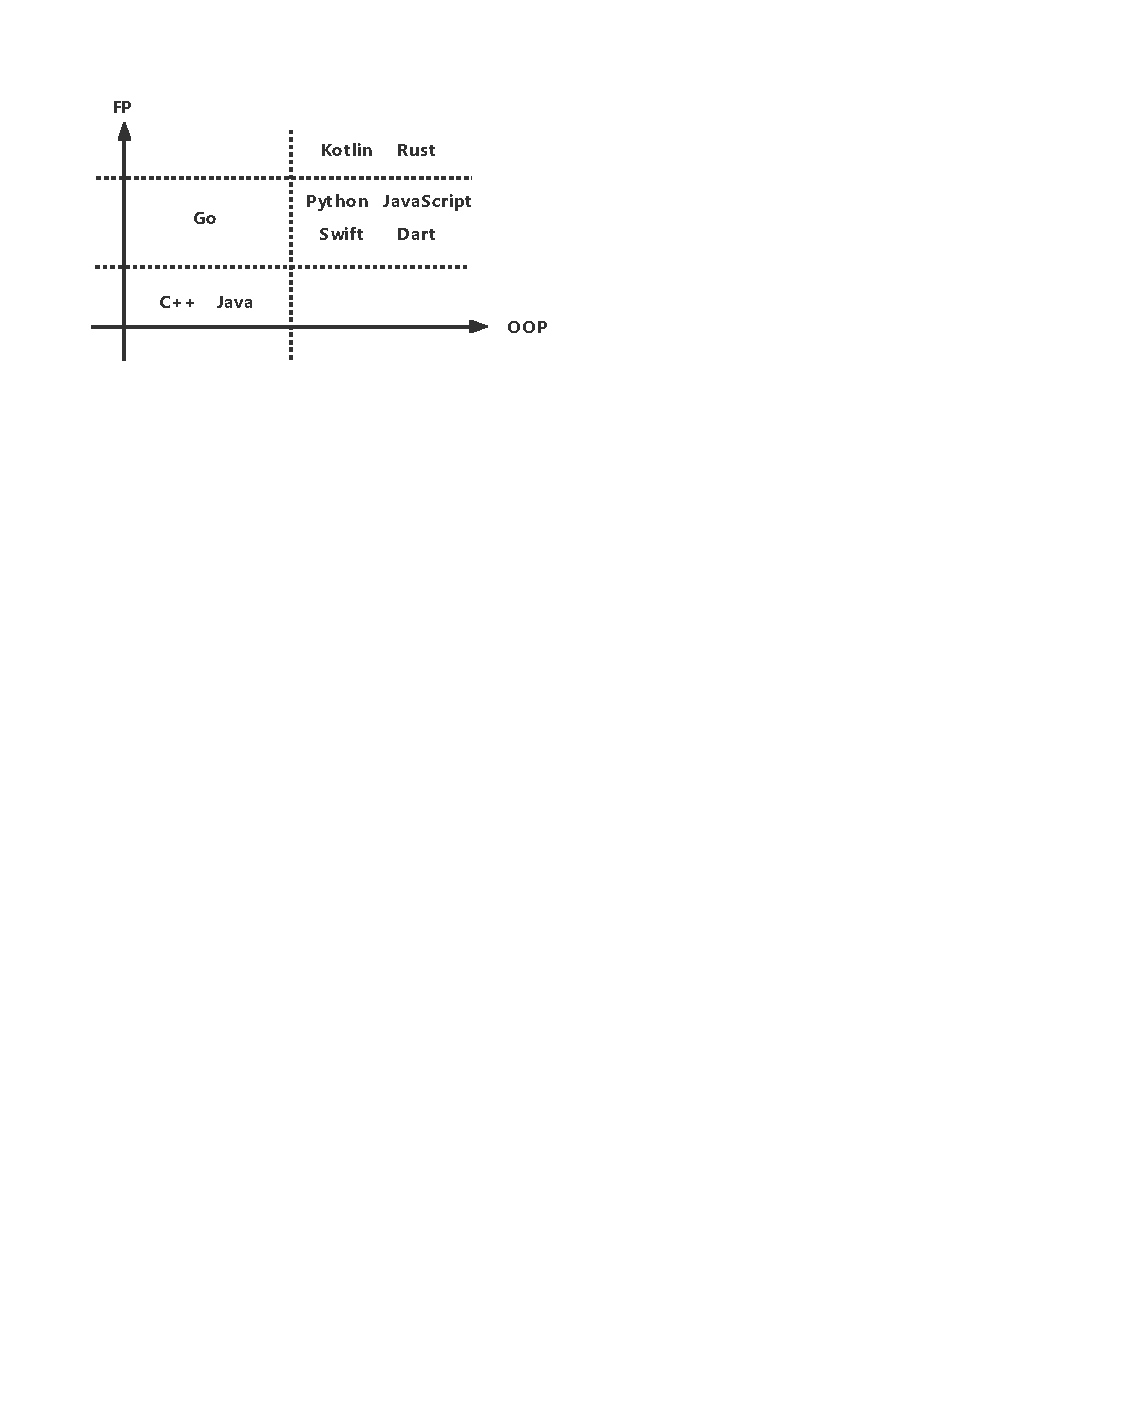
\includegraphics[scale=0.8]{figures/paradigm}}
    \caption{Degree of programming paradigm concept support}
    \label{fig:paradigm}
\end{figure}

The degree to which a programming language supports a programming paradigm is closely related
to the application scenario of the programming language.
Next, we will select a few representative programming languages from Figure~\ref{fig:paradigm} and analyze the
relationship between their programming paradigms and application scenarios.


A typical example is Dart. Its main application scenario is the Web front-end, and it is often used as a support language for the GUI framework Flutter. It is obvious that most of the GUI frameworks we use have a complex inheritance structure. This is because, for GUIs, most of its application scenarios satisfy the Liskov Substitution Principle, i.e., the child type can completely replace the parent type. This is a sufficient condition for using inheritance. Therefore, Dart only provides object-oriented concepts based on inheritance.

The next example is Java, which has weak support for both FP and OOP concepts. In the early years, Java was used for Enterprise development. Later it was used for Web servers, a scenario that required high abstraction of business logic, so Java added the additional concept of FP. However, due to the design of the language itself, the level of support is not high.

Another example is Kotlin, which has better support for both FP and OOP. Its initial application scenario is Android. In order to solve the previous problem that Java was too cumbersome to develop Android applications, Kotlin was designed to add a lot of FP and OOP concepts for the Android application scenario. Not only does it support traditional FP and OOP concepts, but it also makes syntax-level optimizations for these concepts, such as the FP syntactic sugar "trailing lambda" and the OOP delegate syntactic sugar "by". These useful features in turn allow Kotlin to be used in other scenarios, such as server front-ends and back-ends.